\setbeamerfont{block title}{size=\scriptsize}

\section{Advanced package aspects}

\subsection{Licensing report}

\begin{frame}[fragile]{Licensing report: introduction}
  \begin{itemize}
  \item A key aspect of embedded Linux systems is {\bf license
      compliance}.
  \item Embedded Linux systems integrate together a number of
    open-source components, each distributed under its own license.
  \item The different open-source licenses may have {\bf different
      requirements}, that must be met before the product using the
    embedded Linux system starts shipping.
  \item Buildroot helps in this license compliance process by offering
    the possibility of generating a number of {\bf license-related
      information} from the list of selected packages.
  \item Generated using:
\begin{block}{}
\begin{verbatim}
$ make legal-info
\end{verbatim}
\end{block}
  \end{itemize}
\end{frame}

\begin{frame}{Licensing report: contents of {\tt legal-info}}
  \begin{itemize}
  \item \code{sources/} and \code{host-sources/}, all the source files
    that are redistributable (tarballs, patches, etc.)
  \item \code{manifest.csv} and \code{host-manifest.csv}, CSV files
    with the list of {\em target} and {\em host} packages, their
    version, license, etc.
  \item \code{licenses/} and \code{host-licenses/<pkg>/}, the full license text of all {\em
      target} and {\em host} packages, per package
  \item \code{buildroot.config}, the Buildroot \code{.config} file
  \item \code{legal-info.sha256} hashes of all {\em legal-info} files
  \item \code{README}
  \end{itemize}
\end{frame}

\begin{frame}{Including licensing information in packages}
  \begin{itemize}
  \item \code{<pkg>_LICENSE}
    \begin{itemize}
    \item Comma-separated {\bf list of license(s)} under which the
      package is distributed.
    \item Must use SPDX license codes, see
      \url{https://spdx.org/licenses/}
    \item Can indicate which part is under which license (programs,
      tests, libraries, etc.)
    \end{itemize}
  \item \code{<pkg>_LICENSE_FILES}
    \begin{itemize}
    \item Space-separated {\bf list of file paths} from the package
      source code containing the license text and copyright
      information
    \item Paths relative to the package top-level source directory
    \end{itemize}
  \item \code{<pkg>_REDISTRIBUTE}
    \begin{itemize}
    \item Boolean indicating whether the package source code can be
      redistributed or not (part of the \code{legal-info} output)
    \item Defaults to \code{YES}, can be overridden to \code{NO}
    \item If \code{NO}, source code is not copied when generating the
      licensing report
    \end{itemize}
  \end{itemize}
\end{frame}

\begin{frame}[fragile]{Licensing information examples}
  \begin{block}{linux.mk}
\begin{minted}{make}
LINUX_LICENSE = GPL-2.0
LINUX_LICENSE_FILES = COPYING
\end{minted}
  \end{block}

\begin{block}{acl.mk}
\begin{minted}{make}
ACL_LICENSE = GPL-2.0+ (programs), LGPL-2.1+ (libraries)
ACL_LICENSE_FILES = doc/COPYING doc/COPYING.LGPL
\end{minted}
\end{block}

\begin{block}{owl-linux.mk}
\begin{minted}{make}
OWL_LINUX_LICENSE = PROPRIETARY
OWL_LINUX_LICENSE_FILES = LICENSE
OWL_LINUX_REDISTRIBUTE = NO
\end{minted}
\end{block}

\end{frame}

\subsection{Security vulnerability tracking}

\begin{frame}{Security vulnerability tracking}
  \begin{itemize}
  \item Security has obviously become a key issue in embedded systems
    that are more and more commonly connected.
  \item Embedded Linux systems typically integrate 10-100+ open-source
    components $\rightarrow$ not easy to keep track of their potential
    security vulnerabilities
  \item Industry relies on {\em Common Vulnerability Exposure} (CVE)
    reports to document known security issues
  \item Buildroot is able to identify if packages are affected by
    known CVEs, by using the {\em National Vulnerability Database}
    \begin{itemize}
    \item \code{make pkg-stats}
    \item Produces \code{$(O)/pkg-stats.html}, \code{$(O)/pkg-stats.json}
    \end{itemize}
  \item Note: this is limited to known CVEs. It does not guarantee the
    absence of security vulnerabilities.
  \item Only applies to open-source packages, not to your own custom
    code.
  \end{itemize}
\end{frame}

\begin{frame}{Example \code{pkg-stats} output}
  \begin{center}
    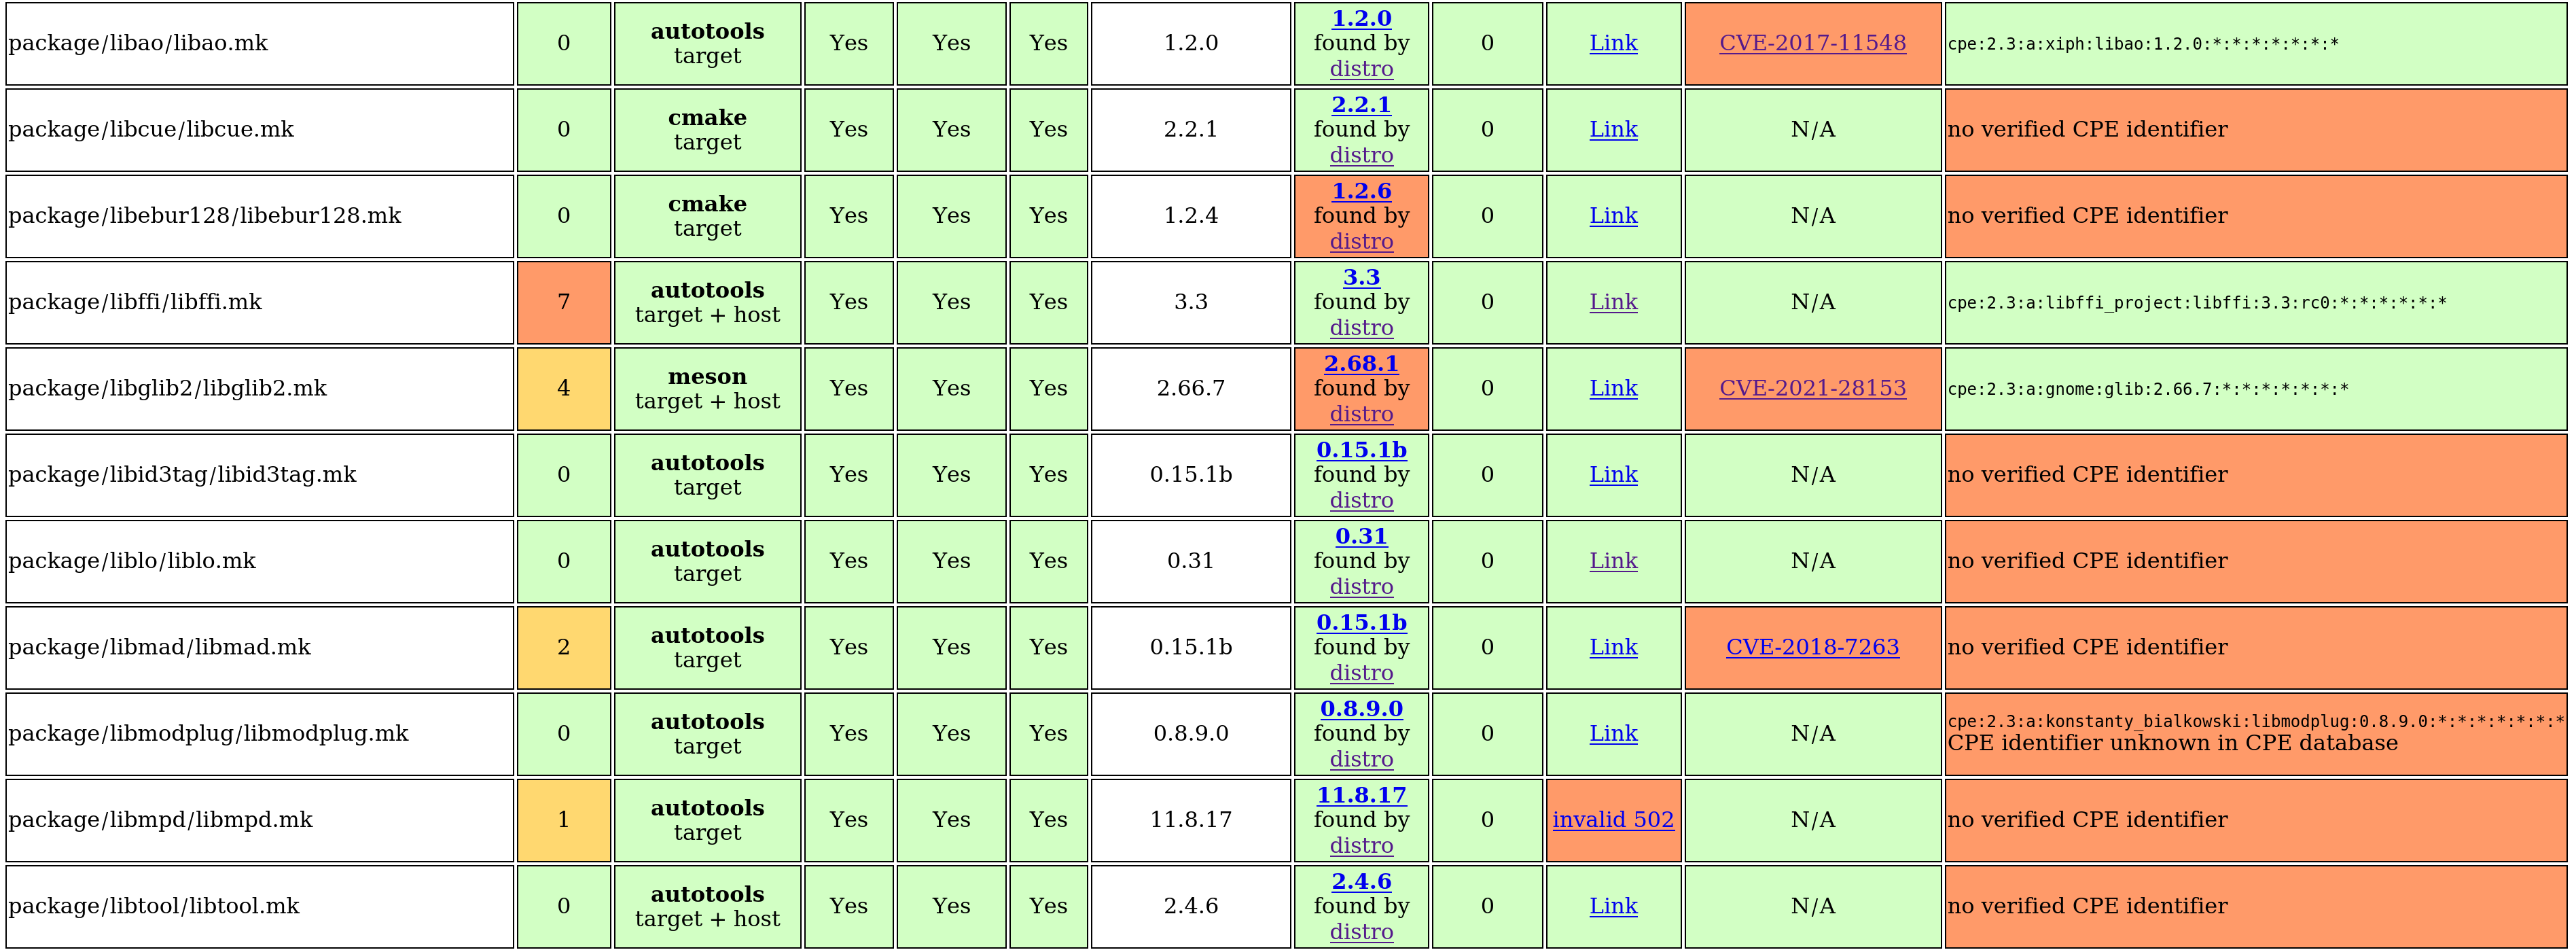
\includegraphics[width=\textwidth]{slides/buildroot-advanced-packages/pkg-stats-output.png}
    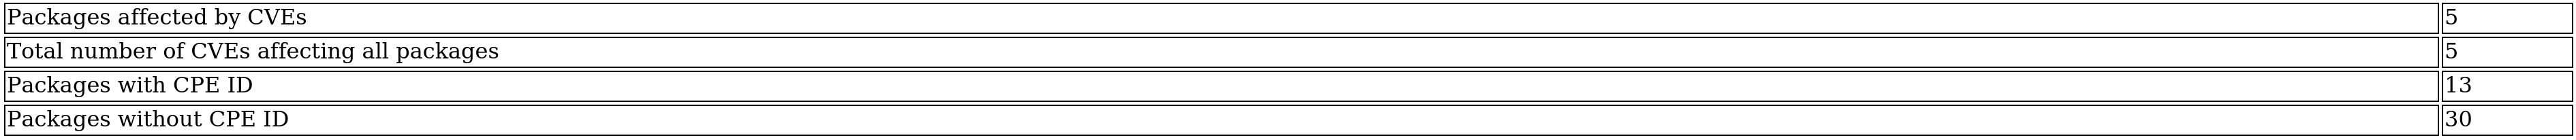
\includegraphics[width=\textwidth]{slides/buildroot-advanced-packages/pkg-stats-output-summary.png}
  \end{center}
\end{frame}

\begin{frame}{CPE: Common Platform Enumeration}
  \begin{itemize}
  \item Concept of {\em Common Platform Enumeration}, which gives a
    unique identifier to a software release
    \begin{itemize}
    \item E.g.: \code{cpe:2.3:a:xiph:libao:1.2.0:*:*:*:*:*:*:*}
    \end{itemize}
  \item By default Buildroot uses:
    \begin{itemize}
    \item \code{cpe:2.3:a:<pkg>_project:<pkg>:<pkg>_VERSION:*:*:*:*:*:*:*}
    \item Not always correct!
    \end{itemize}
  \item Can be modified using:
    \begin{itemize}
    \item \code{<pkg>_CPE_ID_PREFIX}
    \item \code{<pkg>_CPE_ID_VENDOR}
    \item \code{<pkg>_CPE_ID_PRODUCT}
    \item \code{<pkg>_CPE_ID_VERSION}
    \item \code{<pkg>_CPE_ID_UPDATE}
    \end{itemize}
  \item Concept of {\em CPE dictionary} provided by NVD, which
    contains all known CPEs.
    \begin{itemize}
    \item
      \code{pkg-stats} checks if the CPE of each package is known in the {\em CPE dictionary}
    \end{itemize}
  \end{itemize}
\end{frame}

\begin{frame}{NVD CVE-2020-35492 example}
  \begin{center}
    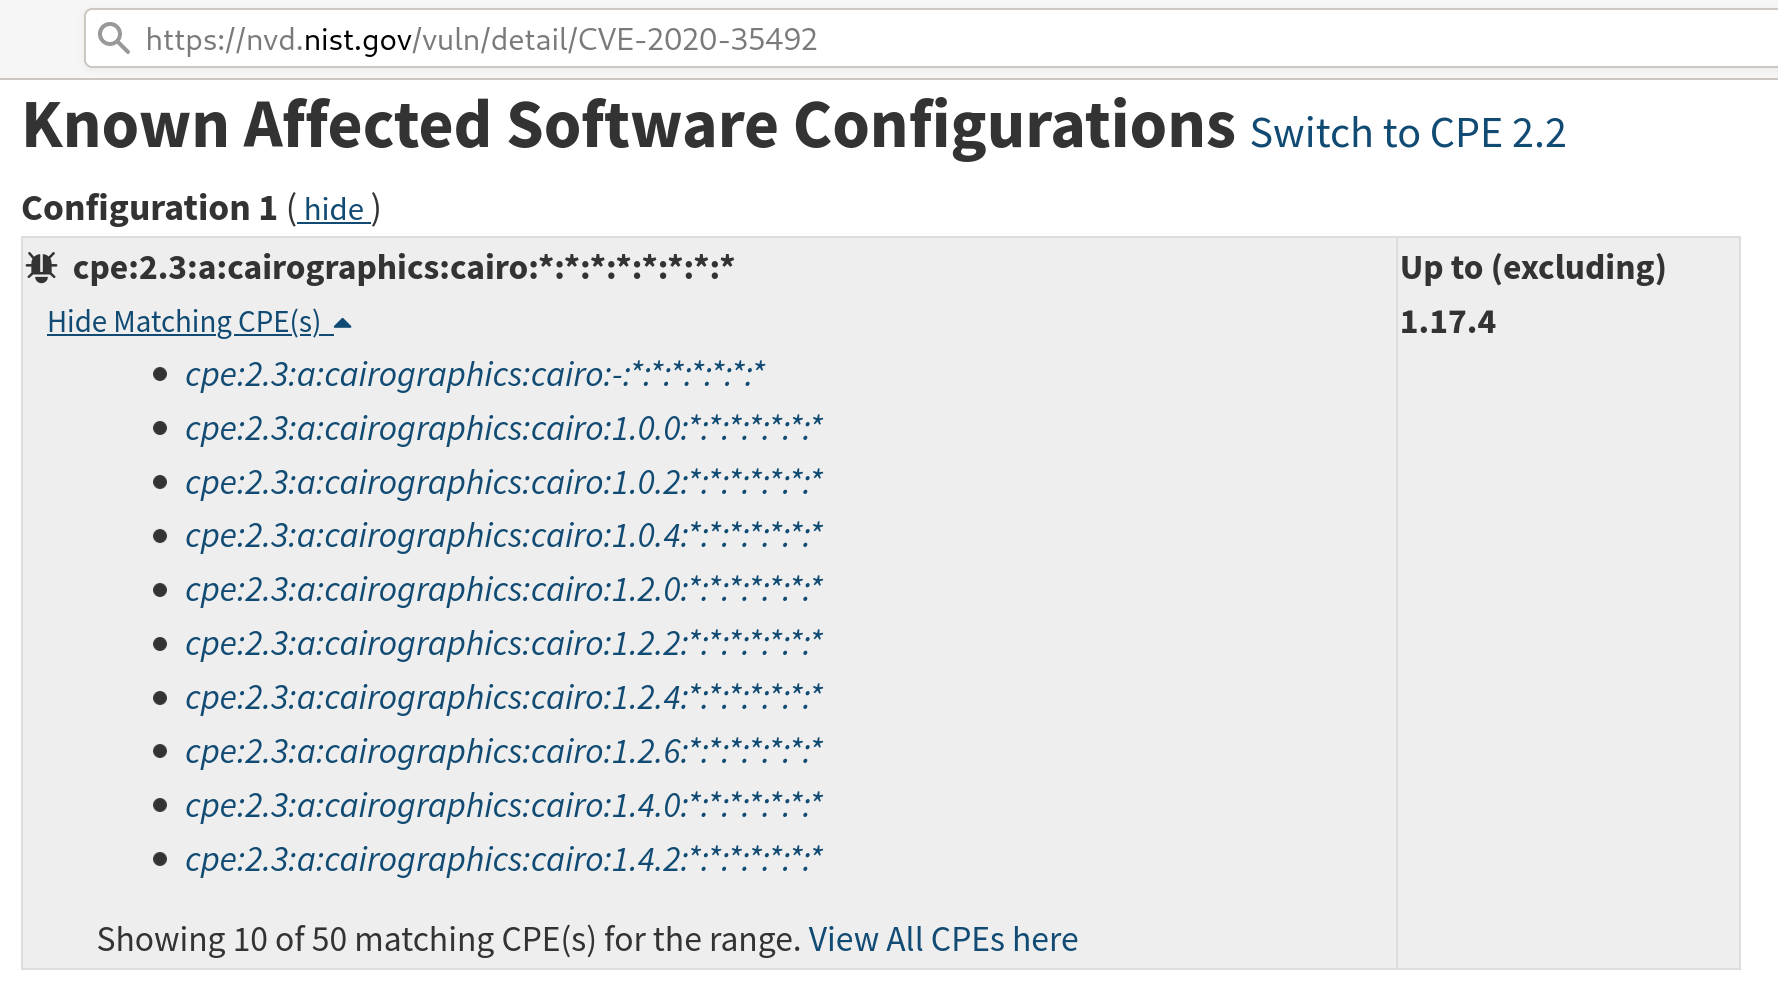
\includegraphics[height=0.8\textheight]{slides/buildroot-advanced-packages/nvd-example.png}
  \end{center}
\end{frame}

\begin{frame}[fragile]{CPE information in packages}

  \begin{block}{\code{package/bash/bash.mk}}
\begin{verbatim}
BASH_CPE_ID_VENDOR = gnu
\end{verbatim}
  \end{block}

  \begin{block}{\code{package/audit/audit.mk}}
\begin{verbatim}
AUDIT_CPE_ID_VENDOR = linux_audit_project
AUDIT_CPE_ID_PRODUCT = linux_audit
\end{verbatim}
  \end{block}

  \begin{block}{\code{linux/linux.mk}}
\begin{verbatim}
LINUX_CPE_ID_VENDOR = linux
LINUX_CPE_ID_PRODUCT = linux_kernel
LINUX_CPE_ID_PREFIX = cpe:2.3:o
\end{verbatim}
  \end{block}

  \begin{block}{\code{package/libffi/libffi.mk}}
\begin{verbatim}
LIBFFI_CPE_ID_VERSION = 3.3
LIBFFI_CPE_ID_UPDATE = rc0
\end{verbatim}
  \end{block}

\end{frame}

\subsection{Patching packages}

\begin{frame}{Patching packages: why?}
  \begin{itemize}
  \item In some situations, it might be needed to patch the source
    code of certain packages built by Buildroot.
  \item Useful to:
    \begin{itemize}
    \item Fix cross-compilation issues
    \item Backport bug or security fixes from upstream
    \item Integrate new features or fixes not available upstream, or
      that are too specific to the product being made
    \end{itemize}
  \item Patches are automatically applied by Buildroot, during the
    {\em patch} step, i.e. after extracting the package, but before
    configuring it.
  \item Buildroot already comes with a number of patches for various
    packages, but you may need to add more for your own packages, or
    to existing packages.
  \end{itemize}
\end{frame}

\begin{frame}{Patch application ordering}
  \begin{itemize}
  \item Overall the patches are applied in this order:
    \begin{enumerate}
    \item Patches mentioned in the \code{<pkg>_PATCH} variable of the
      package \code{.mk} file. They are automatically downloaded
      before being applied.
    \item Patches present in the package directory
      \code{package/<pkg>/*.patch}
    \item Patches present in the {\em global patch directories}
    \end{enumerate}
  \item In each case, they are applied:
    \begin{itemize}
    \item In the order specified in a \code{series} file, if available
    \item Otherwise, in alphabetic ordering
    \end{itemize}
  \end{itemize}
\end{frame}

\begin{frame}[fragile]{Patch conventions}
  \begin{itemize}
  \item There are a few conventions and best practices that the
    Buildroot project encourages to use when managing patches
  \item Their name should start with a sequence number that
    indicates the ordering in which they should be applied.
    \begin{block}{ls package/nginx/*.patch}
      {\scriptsize
\begin{verbatim}
0001-auto-type-sizeof-rework-autotest-to-be-cross-compila.patch
0002-auto-feature-add-mechanism-allowing-to-force-feature.patch
0003-auto-set-ngx_feature_run_force_result-for-each-featu.patch
0004-auto-lib-libxslt-conf-allow-to-override-ngx_feature_.patch
0005-auto-unix-make-sys_nerr-guessing-cross-friendly.patch
\end{verbatim}}
      \end{block}
    \item Each patch should contain a description of what the patch
      does, and if possible its upstream status.
    \item Each patch should contain a \code{Signed-off-by} that
      identifies the author of the patch.
    \item Patches should be generated using
      \code{git format-patch} when possible.
    \end{itemize}
\end{frame}

\begin{frame}[fragile]{Patch example}

\begin{block}{}
{\tiny
\begin{verbatim}
From 81289d1d1adaf5a767a4b4d1309c286468cfd37f Mon Sep 17 00:00:00 2001
From: Samuel Martin <s.martin49@gmail.com>
Date: Thu, 24 Apr 2014 23:27:32 +0200
Subject: [PATCH] auto/type/sizeof: rework autotest to be cross-compilation
 friendly

Rework the sizeof test to do the checks at compile time instead of at
runtime. This way, it does not break when cross-compiling for a
different CPU architecture.

Signed-off-by: Samuel Martin <s.martin49@gmail.com>
---
 auto/types/sizeof | 42 ++++++++++++++++++++++++++++--------------
 1 file changed, 28 insertions(+), 14 deletions(-)

diff --git a/auto/types/sizeof b/auto/types/sizeof
index 9215a54..c2c3ede 100644
--- a/auto/types/sizeof
+++ b/auto/types/sizeof
@@ -14,7 +14,7 @@ END
 
 ngx_size=
 
-cat << END > $NGX_AUTOTEST.c
+cat << _EOF > $NGX_AUTOTEST.c
[...]
\end{verbatim}}
\end{block}

\end{frame}

\begin{frame}{Global patch directories}
  \begin{itemize}
  \item You can include patches for the different packages in their
    package directory, \code{package/<pkg>/}.
  \item However, doing this involves changing the Buildroot sources
    themselves, which may not be appropriate for some highly specific
    patches.
  \item The {\em global patch directories} mechanism allows to specify
    additional locations where Buildroot will look for patches to
    apply on packages.
  \item \code{BR2_GLOBAL_PATCH_DIR} specifies a space-separated list
    of directories containing patches.
  \item These directories must contain sub-directories named after the
    packages, themselves containing the patches to be applied.
  \end{itemize}
\end{frame}

\begin{frame}[fragile]{Global patch directory example}

\begin{block}{Patching {\em strace}}
{\tiny
\begin{verbatim}
$ ls package/strace/*.patch
0001-linux-aarch64-add-missing-header.patch

$ find ~/patches/
~/patches/
~/patches/strace/
~/patches/strace/0001-Demo-strace-change.patch

$ grep ^BR2_GLOBAL_PATCH_DIR .config
BR2_GLOBAL_PATCH_DIR="$(HOME)/patches"

$ make strace
[...]
>>> strace 4.10 Patching

Applying 0001-linux-aarch64-add-missing-header.patch using patch: 
patching file linux/aarch64/arch_regs.h

Applying 0001-Demo-strace-change.patch using patch: 
patching file README
[...]
\end{verbatim}}
\end{block}

\end{frame}

\begin{frame}{Generating patches}
  \begin{itemize}
  \item To generate the patches against a given package source code,
    there are typically two possibilities.
  \item Use the upstream version control system, often {\em Git}
  \item Use a tool called \code{quilt}
    \begin{itemize}
    \item Useful when there is no version control system provided by
      the upstream project
    \item \url{https://savannah.nongnu.org/projects/quilt}
    \end{itemize}
  \end{itemize}
\end{frame}

\begin{frame}{Generating patches: with Git}

  Needs to be done outside of Buildroot: you cannot use the Buildroot
  package build directory.

  \begin{enumerate}
  \item Clone the upstream Git repository\\
    \code{git clone https://...}
  \item Create a branch starting on the tag marking the stable
    release of the software as packaged in Buildroot\\
    \code{git checkout -b buildroot-changes v3.2}
  \item Import existing Buildroot patches (if any)\\
    \code{git am /path/to/buildroot/package/<foo>/*.patch}
  \item Make your changes and commit them\\
    \code{git commit -s -m ``this is a change''}
  \item Generate the patches\\
    \code{git format-patch v3.2}
  \end{enumerate}

\end{frame}

\begin{frame}{Generating patches: with Quilt}

  \begin{enumerate}
  \item Extract the package source code:
    \code{tar xf /path/to/dl/<foo>-<version>.tar.gz}
  \item Inside the package source code, create a directory for patches\\
    \code{mkdir patches}
  \item Import existing Buildroot patches\\
    \code{quilt import /path/to/buildroot/package/<foo>/*.patch}
  \item Apply existing Buildroot patches\\
    \code{quilt push -a}
  \item Create a new patch\\
    \code{quilt new 0001-fix-header-inclusion.patch}
  \item Edit a file\\
    \code{quilt edit main.c}
  \item Refresh the patch\\
    \code{quilt refresh}
  \end{enumerate}

\end{frame}

\subsection{User, permission and device tables}

\begin{frame}[fragile]{Package-specific users}

\begin{itemize}

\item The default skeleton in \code{system/skeleton/} has a number of
  default users/groups.
\item Packages can define their own custom users/groups using the
  \code{<pkg>_USERS} variable:
{\footnotesize
  \begin{block}{}
\begin{verbatim}
define <pkg>_USERS
        username uid group gid password home shell groups comment
endef
\end{verbatim}
  \end{block}}
\item Examples:
  \begin{block}{}
    \begin{minted}[fontsize=\footnotesize]{make}
define AVAHI_USERS
        avahi -1 avahi -1 * - - -
endef
\end{minted}
\end{block}

\begin{block}{}
  \begin{minted}[fontsize=\footnotesize]{make}
define MYSQL_USERS
        mysql -1 nogroup -1 * /var/mysql - - MySQL daemon
endef
  \end{minted}
\end{block}
\end{itemize}

\end{frame}

\begin{frame}[fragile]{File permissions and ownership}

\begin{itemize}

\item By default, before creating the root filesystem images,
  Buildroot changes the ownership of all files to \code{0:0}, i.e.
  \code{root:root}
\item Permissions are preserved as is, but since the build is executed
  as non-root, it is not possible to install setuid applications.
\item A default set of permissions for certain files or directories is
  defined in \code{system/device_table.txt}.
\item The \code{<pkg>_PERMISSIONS} variable allows packages to define
  special ownership and permissions for files and directories:
{\small
  \begin{block}{}
\begin{verbatim}
define <pkg>_PERMISSIONS
name type mode uid gid major minor start inc count
endef
\end{verbatim}
  \end{block}}
\item The \code{major}, \code{minor}, \code{start}, \code{inc} and
  \code{count} fields are not used.

\end{itemize}

\end{frame}

\begin{frame}[fragile]{File permissions and ownership: examples}

  \begin{itemize}
  \item \code{sudo} needs to be installed {\em setuid root}:
  \begin{block}{}
    \begin{minted}[fontsize=\small]{make}
define SUDO_PERMISSIONS
        /usr/bin/sudo f 4755 0 0 - - - - -
endef
\end{minted}
\end{block}

\item \code{/var/lib/nginx} needs to be owned by \code{www-data},
  which has UID/GID \code{33} defined in the skeleton:

\begin{block}{}
  \begin{minted}[fontsize=\small]{make}
define NGINX_PERMISSIONS
        /var/lib/nginx d 755 33 33 - - - - -
endef
\end{minted}
\end{block}

\end{itemize}

\end{frame}

\begin{frame}[fragile]{Devices}
  \begin{itemize}
  \item Defining devices only applies when the chosen \code{/dev}
    management strategy is {\em Static using a device table}. In other
    cases, {\em device files} are created dynamically.
  \item A default set of {\em device files} is described in
    \code{system/device_table_dev.txt} and created by Buildroot in the
    root filesystem images.
  \item When packages need some additional custom devices, they can
    use the \code{<pkg>_DEVICES} variable:
{\small
  \begin{block}{}
\begin{verbatim}
define <pkg>_DEVICES
name type mode uid gid major minor start inc count
endef
\end{verbatim}
  \end{block}}
\item Becoming less useful, since most people are using a dynamic
  \code{/dev} nowadays.
  \end{itemize}
\end{frame}

\begin{frame}[fragile]{Devices: example}

    \begin{block}{xenomai.mk}
      \begin{minted}{make}
define XENOMAI_DEVICES
/dev/rtheap  c  666  0  0  10  254  0  0  -
/dev/rtscope c  666  0  0  10  253  0  0  -
/dev/rtp     c  666  0  0  150 0    0  1  32
endef
      \end{minted}
    \end{block}

\end{frame}

\subsection{Init scripts and systemd unit files}

\begin{frame}{Init scripts, systemd unit files}

\begin{itemize}

\item Buildroot supports several main init systems: {\em sysvinit},
  {\em BusyBox}, {\em systemd}, {\em OpenRC}

\item When packages want to install a program to be started at boot
  time, they need to install a startup script ({\em
    sysvinit}/{\em BusyBox}), a {\em systemd service} file, etc.

\item They can do so using the following variables, which contain a
  list of shell commands.
  \begin{itemize}
  \item \code{<pkg>_INSTALL_INIT_SYSV}
  \item \code{<pkg>_INSTALL_INIT_SYSTEMD}
  \item \code{<pkg>_INSTALL_INIT_OPENRC}
  \end{itemize}

\item Buildroot will execute the appropriate
  \code{<pkg>_INSTALL_INIT_xyz} commands of all enabled packages
  depending on the selected init system.

\end{itemize}

\end{frame}

\begin{frame}[fragile]{Init scripts, systemd unit files: example}

\begin{block}{bind.mk}
  \begin{minted}[fontsize=\scriptsize]{make}
define BIND_INSTALL_INIT_SYSV
        $(INSTALL) -m 0755 -D package/bind/S81named \
                $(TARGET_DIR)/etc/init.d/S81named
endef

define BIND_INSTALL_INIT_SYSTEMD
        $(INSTALL) -D -m 644 package/bind/named.service \
                $(TARGET_DIR)/usr/lib/systemd/system/named.service
endef
  \end{minted}
\end{block}

\end{frame}

\subsection{Config scripts}

\begin{frame}{Config scripts: introduction}
  \begin{itemize}
  \item Libraries not using \code{pkg-config} often install a {\bf
      small shell script} that allows applications to query the
    compiler and linker flags to use the library.
  \item Examples: \code{curl-config}, \code{freetype-config}, etc.
  \item Such scripts will:
    \begin{itemize}
    \item generally return results that are {\bf not appropriate for
        cross-compilation}
    \item be used by other cross-compiled Buildroot packages that use
      those libraries
    \end{itemize}
  \item By listing such scripts in the \code{<pkg>_CONFIG_SCRIPTS}
    variable, Buildroot will {\bf adapt the prefix, header and library
      paths} to make them suitable for cross-compilation.
  \item Paths in \code{<pkg>_CONFIG_SCRIPTS} are relative to
    \code{$(STAGING_DIR)/usr/bin}.
  \end{itemize}
\end{frame}

\begin{frame}[fragile]{Config scripts: examples}

  \begin{block}{libpng.mk}
    \begin{minted}[fontsize=\footnotesize]{make}
LIBPNG_CONFIG_SCRIPTS = \
        libpng$(LIBPNG_SERIES)-config libpng-config
\end{minted}
\end{block}

\begin{block}{imagemagick.mk}
  \begin{minted}[fontsize=\footnotesize]{make}
IMAGEMAGICK_CONFIG_SCRIPTS = \
        $(addsuffix -config,Magick MagickCore MagickWand Wand)

ifeq ($(BR2_INSTALL_LIBSTDCPP)$(BR2_USE_WCHAR),yy)
IMAGEMAGICK_CONFIG_SCRIPTS += Magick++-config
endif
\end{minted}
\end{block}

\end{frame}

\begin{frame}[fragile]{Config scripts: effect}

\begin{block}{Without \code{<pkg>_CONFIG_SCRIPTS}}
{\footnotesize
  \begin{verbatim}
$ ./output/staging/usr/bin/libpng-config --cflags --ldflags
-I/usr/include/libpng16
-L/usr/lib -lpng16
  \end{verbatim}}
\end{block}

\begin{block}{With \code{<pkg>_CONFIG_SCRIPTS}}
{\tiny
  \begin{verbatim}
$ ./output/staging/usr/bin/libpng-config --cflags --ldflags
-I.../buildroot/output/host/arm-buildroot-linux-uclibcgnueabi/sysroot/usr/include/libpng16
-L.../buildroot/output/host/arm-buildroot-linux-uclibcgnueabi/sysroot/usr/lib -lpng16
  \end{verbatim}}
\end{block}

\end{frame}

\subsection{Hooks}

\begin{frame}{Hooks: principle (1)}
  \begin{itemize}
  \item Buildroot {\em package infrastructure} often implement a
    default behavior for certain steps:
    \begin{itemize}
    \item \code{generic-package} implements for all packages the
      download, extract and patch steps
    \item Other infrastructures such as \code{autotools-package} or
      \code{cmake-package} also implement the configure, build and
      installations steps
    \end{itemize}
  \item In some situations, the package may want to do {\bf additional
      actions} before or after one of these steps.
  \item The {\bf hook} mechanism allows packages to add such custom
    actions.
  \end{itemize}
\end{frame}

\begin{frame}{Hooks: principle (2)}
  \begin{itemize}
  \item There are {\bf pre} and {\bf post} hooks available for all
    steps of the package compilation process:
    \begin{itemize}
    \item download, extract, rsync, patch, configure, build, install,
      install staging, install target, install images, legal info
    \item \code{<pkg>_(PRE|POST)_<step>_HOOKS}
    \item Example: \code{CMAKE_POST_INSTALL_TARGET_HOOKS},
      \code{CVS_POST_PATCH_HOOKS}, \code{BINUTILS_PRE_PATCH_HOOKS}
    \end{itemize}
  \item Hook variables contain a list of make macros to call at the
    appropriate time.
    \begin{itemize}
    \item Use \code{+=} to register an additional hook to a hook point
    \end{itemize}
  \item Those make macros contain a list of commands to execute.
  \end{itemize}
\end{frame}

\begin{frame}[fragile]{Hooks: examples}

\begin{block}{bind.mk: remove unneeded binaries}
  \begin{minted}[fontsize=\scriptsize]{make}
define BIND_TARGET_REMOVE_TOOLS
        rm -rf $(addprefix $(TARGET_DIR)/usr/bin/, $(BIND_TARGET_TOOLS_BIN))
endef

BIND_POST_INSTALL_TARGET_HOOKS += BIND_TARGET_REMOVE_TOOLS
  \end{minted}
\end{block}

\begin{block}{vsftpd.mk: adjust configuration}
  \begin{minted}[fontsize=\scriptsize]{make}
define VSFTPD_ENABLE_SSL
        $(SED) 's/.*VSF_BUILD_SSL/#define VSF_BUILD_SSL/' \
                $(@D)/builddefs.h
endef

ifeq ($(BR2_PACKAGE_OPENSSL),y)
VSFTPD_DEPENDENCIES += openssl host-pkgconf
VSFTPD_LIBS += `$(PKG_CONFIG_HOST_BINARY) --libs libssl libcrypto`
VSFTPD_POST_CONFIGURE_HOOKS += VSFTPD_ENABLE_SSL
endif
  \end{minted}
\end{block}

\end{frame}

\subsection{Overriding commands}

\begin{frame}{Overriding commands: principle}

  \begin{itemize}
  \item In other situations, a package may want to completely {\bf
      override} the default implementation of a step provided by a
    package infrastructure.

  \item A package infrastructure will in fact only implement a given
    step {\bf if not already defined by a package}.

  \item So defining \code{<pkg>_EXTRACT_CMDS} or
    \code{<pkg>_BUILD_CMDS} in your package \code{.mk} file will
    override the package infrastructure implementation (if any).

  \end{itemize}

\end{frame}

\begin{frame}[fragile]{Overriding commands: examples}

\begin{block}{jquery: source code is only one file}
\begin{minted}[fontsize=\scriptsize]{make}
JQUERY_SITE = http://code.jquery.com
JQUERY_SOURCE = jquery-$(JQUERY_VERSION).min.js

define JQUERY_EXTRACT_CMDS
        cp $(DL_DIR)/$(JQUERY_SOURCE) $(@D)
endef
\end{minted}
\end{block}

\begin{block}{tftpd: install only what's needed}
\begin{minted}[fontsize=\scriptsize]{make}
define TFTPD_INSTALL_TARGET_CMDS
        $(INSTALL) -D $(@D)/tftp/tftp $(TARGET_DIR)/usr/bin/tftp
        $(INSTALL) -D $(@D)/tftpd/tftpd $(TARGET_DIR)/usr/sbin/tftpd
endef

$(eval $(autotools-package))
\end{minted}
\end{block}

\end{frame}

\subsection{Legacy handling}

\begin{frame}{Legacy handling: {\tt Config.in.legacy}}
  \begin{itemize}
  \item When a \code{Config.in} option is removed, the corresponding
    value in the \code{.config} is silently removed.
  \item Due to this, when users upgrade Buildroot, they generally
    don't know that an option they were using has been removed.
  \item Buildroot therefore adds the removed config option to
    \code{Config.in.legacy} with a description of what has
    happened.
  \item If any of these legacy options is enabled then Buildroot
    refuses to build.
  \end{itemize}
\end{frame}

\subsection{DEVELOPERS file}

\begin{frame}{{\tt DEVELOPERS} file: principle}

  \begin{itemize}
  \item A top-level \code{DEVELOPERS} file lists Buildroot developers
    and contributors interested in specific packages, board {\em
      defconfigs} or architectures.
  \item Used by:
    \begin{itemize}
    \item The \code{utils/get-developers} script to identify to whom a
      patch on an existing package should be sent
    \item The Buildroot {\em autobuilder} infrastructure to notify
      build failures to the appropriate package or architecture
      developers
    \end{itemize}
  \item Important to add yourself in \code{DEVELOPERS} if you
    contribute a new package/board to Buildroot.
  \end{itemize}

\end{frame}

\begin{frame}[fragile]{{\tt DEVELOPERS} file: extract}
\begin{block}{}
{\tiny
\begin{verbatim}
N:      Thomas Petazzoni <thomas.petazzoni@bootlin.com>
F:      arch/Config.in.arm
F:      boot/boot-wrapper-aarch64/
F:      boot/grub2/
F:      package/android-tools/
F:      package/cmake/
F:      package/cramfs/
[...]
F:      toolchain/

N:      Waldemar Brodkorb <wbx@openadk.org>
F:      arch/Config.in.bfin
F:      arch/Config.in.m68k
F:      arch/Config.in.or1k
F:      arch/Config.in.sparc
F:      package/glibc/
\end{verbatim}
}
\end{block}
\end{frame}

\subsection{Virtual packages}

\begin{frame}{Virtual packages}
  \begin{itemize}
  \item There are situations where different packages provide an
    implementation of the same interface
  \item The most useful example is OpenGL
    \begin{itemize}
    \item OpenGL is an API
    \item Each HW vendor typically provides its own OpenGL
      implementation, each packaged as separate Buildroot packages
    \end{itemize}
  \item Packages using the OpenGL interface do not want to know which
    implementation they are using: they are simply using the OpenGL
    API
  \item The mechanism of {\em virtual packages} in Buildroot allows to
    solve this situation.
    \begin{itemize}
    \item \code{libgles} is a virtual package offering the OpenGL ES API
    \item Ten packages are {\em providers} of the OpenGL ES API:
      \code{gpu-amd-bin-mx51}, \code{imx-gpu-viv},
      \code{gcnano-binaries}, \code{mali-t76x}, \code{mesa3d},
      \code{nvidia-driver}, \code{nvidia-tegra23-binaries},
      \code{rpi-userland}, \code{sunxi-mali-mainline}, \code{ti-gfx}
    \end{itemize}
  \end{itemize}
\end{frame}

\begin{frame}{Virtual packages}
  \begin{center}
    \includegraphics[width=\textwidth]{slides/buildroot-advanced-packages/virtual-packages.pdf}
  \end{center}
\end{frame}

\begin{frame}[fragile]{Virtual package definition: Config.in}

\begin{block}{libgles/Config.in}
{\small
\begin{verbatim}
config BR2_PACKAGE_HAS_LIBGLES
        bool

config BR2_PACKAGE_PROVIDES_LIBGLES
        depends on BR2_PACKAGE_HAS_LIBGLES
        string
\end{verbatim}}
\end{block}

\begin{itemize}
\item \code{BR2_PACKAGE_HAS_LIBGLES} is a hidden boolean
  \begin{itemize}
  \item Packages needing OpenGL ES will \code{depends on} it.
  \item Packages providing OpenGL ES will \code{select} it.
  \end{itemize}
\item \code{BR2_PACKAGE_PROVIDES_LIBGLES} is a hidden string
  \begin{itemize}
  \item Packages providing OpenGL ES will define their name as the
    variable value
  \item The \code{libgles} package will have a build dependency on
    this provider package.
  \end{itemize}
\end{itemize}

\end{frame}

\begin{frame}[fragile]{Virtual package definition: {\tt .mk}}

\begin{block}{libgles/libgles.mk}
\begin{minted}{make}
$(eval $(virtual-package))
\end{minted}
\end{block}

\begin{itemize}

\item Nothing to do: the \code{virtual-package} infrastructure takes
  care of everything, using the \code{BR2_PACKAGE_HAS_<name>} and
  \code{BR2_PACKAGE_PROVIDES_<name>} options.

\end{itemize}

\end{frame}

\begin{frame}[fragile]{Virtual package provider}

\begin{block}{sunxi-mali-mainline/Config.in}
{\small
\begin{verbatim}
config BR2_PACKAGE_SUNXI_MALI_MAINLINE
        bool "sunxi-mali-mainline"
        select BR2_PACKAGE_HAS_LIBEGL
        select BR2_PACKAGE_HAS_LIBGLES

config BR2_PACKAGE_PROVIDES_LIBGLES
        default "sunxi-mali-mainline"
\end{verbatim}}
\end{block}

\begin{block}{sunxi-mali-mainline/sunxi-mali-mainline.mk}
\begin{minted}{make}
[...]
SUNXI_MALI_MAINLINE_PROVIDES = libegl libgles
[...]
\end{minted}
\end{block}

\begin{itemize}
\item The variable \code{<pkg>_PROVIDES} is only used to detect if two
  providers for the same virtual package are enabled.
\end{itemize}

\end{frame}

\begin{frame}[fragile]{Virtual package user}

  \begin{block}{qt5/qt5base/Config.in}
{\small
\begin{verbatim}
config BR2_PACKAGE_QT5BASE_OPENGL_ES2
        bool "OpenGL ES 2.0+"
        depends on BR2_PACKAGE_HAS_LIBGLES
        help
          Use OpenGL ES 2.0 and later versions.
\end{verbatim}}
\end{block}

\begin{block}{qt5/qt5base/qt5base.mk}
\begin{minted}[fontsize=\small]{make}
ifeq ($(BR2_PACKAGE_QT5BASE_OPENGL_DESKTOP),y)
QT5BASE_CONFIGURE_OPTS += -opengl desktop
QT5BASE_DEPENDENCIES   += libgl
else ifeq ($(BR2_PACKAGE_QT5BASE_OPENGL_ES2),y)
QT5BASE_CONFIGURE_OPTS += -opengl es2
QT5BASE_DEPENDENCIES   += libgles
else
QT5BASE_CONFIGURE_OPTS += -no-opengl
endif
\end{minted}
\end{block}

\end{frame}

\setuplabframe
{Advanced packages}
{
  \begin{itemize}
  \item Package an application with a mandatory dependency and an
    optional dependency
  \item Package a library, hosted on GitHub
  \item Use {\em hooks} to tweak packages
  \item Add a patch to a package
  \end{itemize}
}
